\setchapterpreamble[u]{\margintoc}
\chapter{Introduction in English}
\labch{intro_english}

% This thesis deals with dependent type theory, a discipline that lies at the 
% intersection of mathematics, formal logic and computer science.

% What is dependent type theory about?
% % 
% The answer is simple: it is high-level, functional programming language with a
% type system that is so expressive that we can use it to express complex
% logical constraints, ensuring that programs are correct simply by virtue of 
% being well-typed.
% % 
% Well, not really. In fact dependent type theory is closer to a foundation for 
% mathematics, one that is more faithful to the mathematical intuition than 
% first-order set theory.
% % 
% But that leaves out the most interesting part of the picture!
% % 
% Type theory is a mathematical object in its own right, a sophisticated 
% algebraic theory whose class of models 

\section{Equality in Intensional Type Theory}

If you have ever used a proof assistant based on intensional type theory such as
\Coq, \Agda or {\Lean}---and there is a good chance that you have if you are 
reading this thesis---then you probably know that equality can be a real headache.

On the one hand we have the \emph{definitional} equality (also called conversion), which records the 
equations that the proof assistant handles silently for us.
% 
\sideremark{In proof assistants based on ZF set theory such as Metamath,
  the theorem \( 2+2=4 \) does requires a proof. Although it is elementary,
  this proof involves a surprising amount of auxiliary lemmas!}
% 
For instance, the terms \( 2+2 \) and \( 4 \) are definitionally equal, meaning that we 
can use them interchangeably in our proofs without having to worry about 
proving their equality by hand.
% 
In a dependently typed setting, this minimal amount of automation is absolutely vital; 
lest we have to insert explicit coercions every time we want to say, use a term 
of type \( \mathsf{Vector}\ (2+2) \) as a term of type \( \mathsf{Vector}\ 4 \).

But unfortunately not everything is a natural 
number, and mathematical proofs
frequently deal with equalities between infinitary objects such as functions and 
sets.
% 
And of course there is no algorithm that can decide whether
two functions of type \( \Nat \to \Nat \) are pointwise equal.
% 
Thus in practice, the definitional equality is limited to 
\( \beta / \eta / \iota \) equalities, with perhaps some extensions
such as \Agda's rewrite rules~\sidecite{taming_of_the_rew}.

Since the system will not be able to fully automate all equalities away, 
we need facilities to reason about them.
% 
This is why intensional type theories provide a second notion of equality, 
called the \emph{propositional} equality. 
% 
Contrary to the definitional equality, this one is available internally in
the language of type theory, so that we may use it to state and prove theorems.
% 
In all three major proof assistants based on type theory, the propositional 
equality is implemented as an inductive type, after the pioneer work of Martin-Löf~\sidecite{MartinLoef75}.
% 
\sideremark{The propositional equality \( \Indeq{A}{t}{u} \) is a type, while the
  definitional equality \( \eqtm{\Gamma}{t}{u}{A} \) is a typing judgment.}
\begin{mathpar}
  \inferrule{\tyty{\Gamma}{A}
			\\ \tytm{\Gamma}{t}{A}
			\\ \tytm{\Gamma}{u}{A}}
			{\tyty{\Gamma}{\Indeq{A}{t}{u}}}
  \and
  \inferrule{\tyty{\Gamma}{A}
			\\ \tytm{\Gamma}{t}{A}}
			{\tytm{\Gamma}{\indrefl{t}}{\Indeq{A}{t}{t}}}
\end{mathpar}
\begin{mathpar}
  \inferrule{\tyty{\Gamma}{A}
			\\ \tytm{\Gamma}{t}{A}
			\\ \tytm{\Gamma}{B}{\Depfun{A}{\Fun{t =_A x}{\Univ}}}
			\\ \tytm{\Gamma}{u}{B\ t\ \mathsf{refl}_t}
			\\ \tytm{\Gamma}{t'}{A}
			\\ \tytm{\Gamma}{e}{t =_A t'}}
			{\tytm{\Gamma}{\mathsf{J}(A,t,B,u,t',e)}{B\ t'\ e}}
\end{mathpar}
\begin{mathpar}
  \inferrule{[...]}
			{\red{\Gamma}{\mathsf{J}(A,t,B,u,t,\mathsf{refl}_t)}{u}{B\ t\ \mathsf{refl}_t}}
\end{mathpar}

These few rules are enough to define an equivalence relation that contains
the definitional equality, can be used to rewrite terms and can be used to coerce
between equal types.
%  (using the \( \mathsf{J} \) operator).

An important difference with the common practice of mathematics is the 
attachment to the Curry-Howard correspondence between proofs and programs:
equality is a \emph{type}, and equality proofs are \emph{programs}.
% 
As such, equality proofs are first class values like the natural numbers
or the functions, and we can reason about them or evaluate them just as well.

\subsection{Types and Propositions}

While the possibility to evaluate proofs is a core tenet of the Curry-Howard
doctrine, the typical equality proof does not exhibit a very interesting 
computational behavior. 
% 
The term \( \indJ{A}{t}{P}{u}{t'}{e} \) just waits for \( e \) to reduce to
a proof by reflexivity, in which case \( t \) and \( t' \) are convertible and
the whole term can simply evaluate to \( u \). 

As a consequence, the programs 
\defnote{extracted}{Extraction produces a program in an external programming 
  language by erasing some type information.} 
from proofs that use equational reasoning  tend to spend a lot of time passing 
around equality proofs just to end up discarding them.
% 
This less-than-ideal state of affairs led the \Coq proof assistant to introduce
a special sort \( \varProp \) for types whose proofs are to be erased during 
program extraction~\sidecite{letouzey04}.
% 
By putting the propositional equality in \( \varProp \) along with the other logical 
constraints that do not play any role in computation, \Coq recovers reasonably good 
performances for extracted programs. 

Technically this is a bit of an infrigement of the Curry-Howard discipline, as \( \varProp \) 
effectively re-introduces a separation between propositions and data.
% 
But make no mistake: proofs of propositions still play their normal role in computations, and in 
particular they may block the evaluation of open terms. 
% 
It is only when we extract an \emph{external} program that propositions become irrelevant.

The \Lean proof assistant goes a step further and introduces the sort 
% 
\sideremark{The \Lean community uses the name \( \varProp \) for the sort of
  strict propositions, but we will use \( \varsProp \) to avoid confusion with
  non-strict propositions.}
% 
\( \varsProp \) for \emph{strict propositions}~\sidecite{lean}.
% 
% \sideremark{Nowadays strict propositions are also available in \Coq and
%   \Agda, although they do not use them for the propositional equality.}
% 
Contrary to \Coq's propositions, the strict propositions are proof-irrelevant, 
meaning that any two inhabitants of a strict proposition \( A \) are 
definitionally equal simply by virtue of having type \( A \).
% 
\[
\inferrule{\tytm{\Gamma}{A}{\varsProp} \\ \tytm{\Gamma}{t, u}{A}}{\eqtm{\Gamma}{t}{u}{A}}
\]

Putting the propositional equality in \( \varsProp \) is not exactly innocuous.
% 
It means that any proof of propositional equality between two convertible 
terms is now undistinguishable from a proof by reflexivity since they have the 
same type.
% 
In other words \Lean satisfies a strict version of the principle of \emph{uniqueness 
of identity proofs} (UIP).

Now non-reflexive equality proofs can't block computation anymore: the term
\( \indJ{A}{t}{P}{u}{t}{e} \) is convertible to 
\( \indJ{A}{t}{P}{u}{t}{\indrefl{t}} \), which should reduce!
% 
As a consequence, the \( J \) eliminator of \Lean reduces whenever it is applied to 
definitionally equal terms.
\begin{mathpar}
  \inferrule[J-conv]{[...] \\ \eqtm{\Gamma}{t}{t'}{A}}
			{\red{\Gamma}{\mathsf{J}(A,t,B,u,t',e)}{u}{B\ t'\ e}}
      \ilabel{infrule:J-conv}
\end{mathpar}

But while this rule is logically sound, Abel and Coquand showed that it leads to a 
failure of normalization for open terms~\cite{lmcs:6606}.
% 
\sideremark{It is known that \Lean's definitional equality is undecidable for
  other, independent reasons~\cite{gilbert:hal-01859964}. But this certainly
  did not prevent the \Lean community from developing a large amount of 
  mathematics.}
% 
Since the algorithms we use to check for convertibility rely on normalization, it 
follows that adding rule~\nameref{infrule:J-conv} breaks our decision procedures
for the definitional equality.
% 
As noted by Abel and Coquand, it is not clear whether this stems from a 
fundamental incompatibility between impredicative strict propositions and the 
propositional equality, or if a more clever strategy could solve this problem.

\subsection{Impredicativity}

In dependent type theory, a sort is said to be \emph{impredicative} if it is 
closed under dependent products over any index type. 
% 
For instance the sort of \Coq propositions is impredicative, because for all 
types \( A \) and functions \( \tm{B}{A \to \varProp} \) the dependent product 
\( \Depfun{A}{B\ x} \) is in \( \varProp \).
% The same goes for \Lean's strict propositions.

Impredicativity allows some amount of self-reference into the type system: 
we can use it to form a proposition \( P \) which quantifies over the type 
\( \varProp \) of all propositions, a type that contains \( P \).
% 
A classic example is the impredicative encoding of the false proposition, 
whose inhabitants can be eliminated into any other proposition:
\[
\bot \enskip := \enskip \Depfun[X]{\varProp}{X} \enskip : \enskip \varProp
\]

Compare this situation with the \emph{predicative} hierarchy 
$(\varType_i)_{i \in \Nat}$ 
% 
\sideremark{In the case of \Coq the predicative universes are technically not
  indexed by integers, but the system maintains a graph of level constraints that
  effectively does the same job.}
% 
of non propositional types.
In the non-propositional world, dependent products are forced to inhabit a 
universe level that is higher than both the level of their domain and the level
of their codomain:
% 
given a type \( A : \varType_i \) and a function \( {\tm{B}{A \to \varType_j}} \), 
their dependent product \( \Depfun{A}{B\ x} \) is in 
\( \varType_{\mathsf{max}(i,j)} \).
 
Predicativity removes the possibility for self-reference: if we try to 
replicate the encoding of the false proposition in \( \varType_0 \), the
resulting type lands in the next universe.
\[
\Depfun[X]{\varType_0}{X} \enskip : \enskip \varType_1
\]

Playing with self-reference is always a dangerous game: 
logical antinomies born of Russell's paradox are lurking in the shadows, and 
might catch us if we get a bit too greedy with our logical principles. 
% 
For instance, Berardi's paradox shows that having excluded middle and booleans
with large elimination in \( \varProp \) is inconsistent.
% 
Impredicativity also plays a central role in the non-normalizing term
that Abel and Coquand derived from rule~\nameref{infrule:J-conv}~\sidecite{lmcs:6606}.

In counterpart to this fragility, impredicativity greatly increases the
expressive power of our logical system, and allows us to formulate important 
mathematical constructions such as Tarski's fixed point theorem or nontrivial 
complete lattices~\sidecite{paco}.
% 
Plus some theorems such as the normalization of System F outright cannot be 
proved in a predicative theory.

Different proof assistants have adopted different attitudes toward 
impredicativity.
% 
On the one hand,
% 
\sideremark{Back in the day the \Coq proof assistant used impredicative sorts
  for both computational data and proofs, but the development team switched to a 
  theory that is more compatible with classical mathematics.}
% 
\Coq and \Lean both have embraced impredicativity for their sort for propositions, 
which cohabits with a predicative universe hierarchy used for the computationally 
relevant types~\sidecite{Coq:manual,lean}.
%
On the other hand, the \Agda proof assistant prefers not to support impredicativity 
at all and uses two predicative hierarchies instead, 
one for strict propositions and one for types~\sidecite{agda261}.

\section{Recovering Extensionality in Intensional Type Theory}

The basic propositional equality that we defined as an inductive type does 
not quite meet the standards of mathematical reasoning.
% 
In mathematics, two functions are considered equal when they agree on all 
inputs---this is the principle of \emph{function extensionality}---but
% 
\sideremark{In particular, it is not possible to prove that the functions
\( {\lambda\ n\ .\ n+1} \) and \( {\lambda\ n\ .\ 1+n} \) are equal.}
% 
this principle is not derivable for the propositional equality in 
intensional type theory.
\[
  \Indeq{A \to B}{f}{g} \quad \xcancel{\longleftrightarrow} \quad \Depfun{A}{\Indeq{B}{f\ x}{g\ x}}
\]

In fact, we can show that all proofs of propositional equality in an empty 
context reduce to the definitional equality.
% 
This is a straightforward consequence of the normalization of well-typed terms:
the sole closed normal form for an equality proof is \( \indrefl{t} \), which
only type-checks if the two endpoints are convertible.
% 
And as we explained earlier, the definitional equality does not handle pointwise
equality of functions.

% All in all, the propositional equality is better thought of as an equality 
% between programs than as an equality between mathematical objects.

Developing sophisticated mathematics without the principle of 
function extensionality is not an easy task.
Consequently, the community has explored several options to recover a more 
conventional equality throughout the years.

\paragraph*{Extensionality axioms}
% 
The most obvious way to recover a missing reasoning principle is simply to
postulate it as an axiom. 
% 
\sideremark{Note that in \Coq and \Lean it is still possible to extract a program 
  from a proof that postulates function extensionality, because the axiom
  is erased during extraction.}
% 
For instance, the axiom \textsf{functional\_extensionality\_dep} is available 
in \Coq's standard library.
% 
The downside of using axioms is that they do not play so well with the 
computational properties of intensional type theory:
% 
% intensional type theory is built around the proofs-as-programs correspondence, 
% and every existence proof doubles as an algorithm that computes the witness
% of existence.
% 
applying the \( J \) eliminator to an equality obtained \textit{via} an axiom
will only result in a stuck term.

\paragraph*{Setoids}
% 
A standard technique to recover extensionality principles without breaking the
proofs-as-programs correspondance is to use \emph{setoids}~\sidecite{hofmann95},
\ie to replace types with pairs \( (|A|, e_A) \) of a carrier type \( |A| \)
and an equivalence relation \( e_A \) on \( |A| \) 
(the \emph{setoid equality} of \( A \)).
% 
We then restrict our attention to functions that preserve the setoid equality, 
and we bake function extensionality into the setoid equality of function types.

Working with setoids is not exactly pleasant, as we need to supplement every
definition with bureaucratic proofs of preservation of the setoid equalities,
even though all available constructs in type theory do respect function 
extensionality~\sidecite{Altenkirch99}.
% 
Basically, we need to do the work of a compiler by hand.
% 
The \Coq proof assistant provides some automation to deal with setoids through 
tactics, but these solutions do not scale painlessly to large developments---to 
the point that the community has coined the term \emph{setoid hell} to refer 
to these issues.

\paragraph*{Alternative type theories}
% 
Since extensionality axioms are problematic because they block 
computation, type theorists have explored numerous ways to extend intensional
type theory with new computational rules that handle the desired axioms.
% 
The most successful lines of work can be roughly divided into two groups: the 
ones that replace the inductive propositional equality with an \emph{observational equality}, 
and the ones that replace it with a \emph{univalent equality}.
% 
% In the first half of this thesis, we will restrict our attention to the first 
% group. The univalent equality is at the center of the second half, and we 
% invite the interested reader to have a look at \cref{ch:hott}.

\subsection{Observational Equality}

The observational equality has its roots in the setoid model of type theory, 
developed by Altenkirch after some explorations by Hofmann~\cite{hofmann95,altenkirch99}.
% 
By interpreting types as setoids, Altenkirch was able to model
\defnote{ITT+funext}{ITT+funext stands for intensional type theory extended 
  with function extensionality.}
in an intensional type theory extended with strict propositions.
% 
Since these strict propositions do not conflict with the proofs-as-programs 
interpretation, the setoid model provides a way to evaluate proofs that use a 
function extensionality axiom by evaluating their interpretation.

The central ingredient of the setoid model is the interpretation of the 
universe.
% 
Constructing a setoid of small setoids seemed difficult at first, because 
the collection of all small setoids does not have a natural setoid equality;
but this can be solved by using an 
\defnote{inductive-recursive}{Induction-recursion is a powerful principle that 
  allows us to define an inductive type \( A \) simultaneously with functions
  defined by recursion on \( A \).}
universe of codes on which the setoid equality and type coercion operators are 
defined by recursion.

Following this first step, Altenkirch McBride and 
Swierstra~\sidecite{altenkirchAl:plpv2007} developed observational 
type theory (OTT), an extension of intensional type theory that brings the main 
insights of the setoid model back to the world of syntax:
% 
OTT introduces a new primitive operator called the \emph{observational equality} that 
equips every type with a setoid structure defined by recursion on the universe.
% 
The result is a type theory that supports the principles of UIP and function 
extensionality, and Altenkirch \etal prove that normalization of OTT terms 
follows from a conjectured normalization result for type theory with 
induction-recursion.

The observational equality has seen some new and exciting developments in recent 
years, such as the work of Sterling \etal who revisit it under the lens of 
cubical type theory~\sidecite{sterling-angiuli-gratzer:2022} or the setoid
type theory of Altenkirch \etal~\sidecite{Altenkirch2019}.
% 
Still, observational type theory has yet to reach a level of maturity 
comparable to that of univalent type theories.
% 
In particular, there is still no support for the observational equality in
major proof assistants, despite some significant work in that 
direction~\sidecite{mcbride-autopsy}.

\subsection{Univalent Equality}
\label{sec:univalence}

The other line of work is more recent and takes its roots in
Voevodsky's \emph{univalence axiom}~\sidecite{kapulkin2012simplicial,hottbook}.
\[
(A =_{\varType} B) \enskip \simeq \enskip  (A \simeq B)
\]
The univalence axiom gives a new meaning to the equality between types: 
% 
\sideremark{The correct definition of an isomorphism between types is somewhat 
  subtle, so we will simply take it as granted for the time being.}
% 
a witness of equality between \( A \) and \( B \) is now the same as an element of the type 
\( A \simeq B \) of \emph{isomorphisms} between \( A \) and \( B \). 
% 
This can be seen as an extensionality principle for the universe of types, and
adding it to intensional type theory has far reaching consequences. 
In particular, univalence implies the principle of function extensionality.

\paragraph*{Homotopy Type Theory}
% 
The univalence axiom departs from the standard mathematical usage of equality, 
in that equality can no longer be a proposition since it now contains essential
computational information. 
% 
For instance there are two distinct automorphisms of the type of booleans 
---one corresponding to the identity and the other to negation---and transporting along
the identity is not the same as transporting along negation.
\sideremark{Transporting along an isomorphism amounts to an application of the
  isomorphism, up to a propositional equality.}
\[
\begin{split}
\indJ{\varType}{\mathsf{Bool}}{\lambda X\ .\ X}{\mathsf{true}}{\mathsf{Bool}}{\mathsf{id}} & \enskip =_{\mathsf{Bool}} \enskip \mathsf{true} \\
\indJ{\varType}{\mathsf{Bool}}{\lambda X\ .\ X}{\mathsf{true}}{\mathsf{Bool}}{\mathsf{neg}} & \enskip =_{\mathsf{Bool}} \enskip \mathsf{false}
\end{split}
\]

Thus when we use the univalence axiom, we must accept that types now contain 
important information in their equality types. 
% 
But these equality types also contain information in their own equality types,
and so on. 
% 
We end up with infinite towers of relevant equality types, all contained in the
data of a type.

\begin{figure}[!h]
  \tikzset{every picture/.style={line width=0.75pt}} %set default line width to 0.75pt        
  \begin{minipage}{0.4\textwidth}
    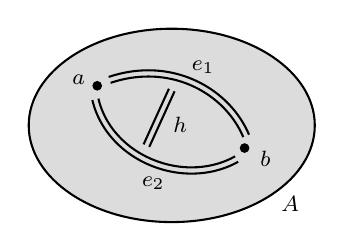
\begin{tikzpicture}[x=0.75pt,y=0.75pt,yscale=-1,xscale=1,roundnode/.style={circle, fill=black, inner sep=0pt, minimum size=3.5pt}]
    %uncomment if require: \path (0,300); %set diagram left start at 0, and has height of 300

    %Shape: Ellipse [id:dp3643970014729053] 
    \draw  [fill={rgb, 255:red, 220; green, 220; blue, 220 }  ,fill opacity=1 ] (4,52.08) .. controls (4,26.36) and (34.86,5.5) .. (72.92,5.5) .. controls (110.98,5.5) and (141.83,26.36) .. (141.83,52.08) .. controls (141.83,77.81) and (110.98,98.67) .. (72.92,98.67) .. controls (34.86,98.67) and (4,77.81) .. (4,52.08) -- cycle ;
    %Curve Lines [id:da06896022650610556] 
    \draw    (42.51,28.73) .. controls (49.06,26.53) and (55.48,25.53) .. (61.61,25.53) .. controls (81.63,25.53) and (98.59,36.2) .. (107.29,50.91) .. controls (108.37,52.74) and (109.33,54.63) .. (110.14,56.57)(43.46,31.57) .. controls (49.69,29.48) and (55.78,28.53) .. (61.61,28.53) .. controls (80.48,28.53) and (96.5,38.56) .. (104.71,52.44) .. controls (105.72,54.15) and (106.61,55.92) .. (107.38,57.73) ;
    %Curve Lines [id:da08140854638152761] 
    \draw    (37.58,39.19) .. controls (41.3,54.8) and (53.94,65.9) .. (68.57,70.27) .. controls (72.96,71.58) and (77.53,72.28) .. (82.1,72.31) .. controls (82.22,72.31) and (82.34,72.31) .. (82.46,72.31) .. controls (89.71,72.31) and (96.96,70.63) .. (103.45,66.99)(34.66,39.89) .. controls (38.64,56.55) and (52.07,68.48) .. (67.72,73.14) .. controls (72.37,74.53) and (77.23,75.28) .. (82.08,75.31) .. controls (82.2,75.31) and (82.33,75.31) .. (82.46,75.31) .. controls (90.22,75.31) and (97.97,73.5) .. (104.92,69.61) ;
    %Straight Lines [id:da7856762818241472] 
    \draw    (74.28,35.66) -- (62.08,62.46)(71.55,34.42) -- (59.35,61.22) ;

    \node[roundnode] (B0) at (37,33) {};
    \node (C0) at (28,30) {\footnotesize{$a$}};
    \node[roundnode] (B1) at (108,63) {};
    \node (C1) at (118,68) {\footnotesize{$b$}};
    \node (C2) at (88,24) {\footnotesize{$e_1$}};
    \node (C3) at (64,80) {\footnotesize{$e_2$}};
    \node (C4) at (77,52) {\footnotesize{$h$}};
    \node (C5) at (130,90) {\footnotesize{$A$}};
    \end{tikzpicture}
  \end{minipage}
  \begin{minipage}{0.4\textwidth}
  \[
    \begin{array}{l}
      A : \varType_i \\
      a : A \\
      b : A \\
      e_1 : \Indeq{A}{a}{b} \\
      e_2 : \Indeq{A}{a}{b} \\
      h : \Indeq{(\Indeq{A}{a}{b})}{e_1}{e_2}
    \end{array}
  \]
  \end{minipage}
  \caption{Graphical representation of a type with inhabitants and equalities}
\end{figure}
 
All in all, these types do not really resemble sets anymore. 
% 
Voevodsky noticed that they are much closer to \emph{weak \( \infty \)-groupoids}, 
a higher categorical gadget that plays an important role in homotopy theory, 
the branch of math that studies spaces and their deformations.
% 
This is the starting point of \emph{homotopy type theory} (HoTT), a far-reaching analogy
between homotopy theory and intensional type theory with the univalence 
axiom~\cite{hottbook}.

In HoTT, we think of types as spaces. Inhabitants of a type 
play the role of its points, equalities between two terms correspond to paths
between the points, equalities between two equalities are continuous
deformations between the corresponding paths, and so on. 
% 
Naturally, functions between types are continuous in that they preserve
equalities, and isomorphisms correspond to homotopy equivalences.

Homotopy type theory also extends the notion of inductive type to 
\emph{higher inductive types} (HITs), which feature constructors for paths/equalities
in addition to constructors for elements.
% 
HITs provide a variety of basic spaces, such as the circle, the sphere and
the torus, but also a notion of quotient types.
% 
\sideremark{This definition of the \textsf{circle} type might be surprising,
  as it looks nothing like the expected space
  \( \{ (x, y) \in \mathbb{R}^2\ |\ x^2 + y^2 = 1 \} \).
  This is because types in HoTT are not \emph{topological} spaces, but rather
  synthetic spaces built out of points, paths and higher dimensional faces.
  As such, the \textsf{circle} is freely generated by a base point and a path
  from that base point to itself.}
\[
\begin{array}{l}
\mathsf{Inductive}\enskip\mathsf{circle} : \varType_0\enskip := \\
\sep \quad \mathsf{base} \enskip : \enskip \mathsf{circle}\\
\sep \quad \mathsf{loop} \enskip : \enskip \Indeq{\mathsf{circle}}{\mathsf{base}}{\mathsf{base}} \\
\end{array}
\]
\[
\begin{array}{l}
\mathsf{Inductive}\enskip\mathsf{quotient}\ (A : \varType_i)\ (R : A \to A \to \varType_i) : \varType_i\enskip := \\
\sep \quad \mathsf{emb} \enskip : \enskip A \to \mathsf{quotient}\ A\ R \\
\sep \quad \mathsf{quo} \enskip : \enskip \Depfun[a\ b]{A}{R\ a\ b \to \Indeq{...}{\mathsf{emb}\ a}{\mathsf{emb}\ b}} \\
\end{array}
\]

Using higher inductive types and the univalence axiom it becomes possible to 
prove a surprising amount of classical results from homotopy theory, rephrased
to talk about types and equality:
% 
in his PhD thesis, Brunerie managed to show that the fourth homotopy group of
the three-dimensional sphere has two elements~\sidecite{Brunerie16}.
% 
Since then, the HoTT community has developed extensive libraries of formalized
univalent mathematics in \Coq~\sidecite{Bauer:2017:HLF:3018610.3018615} and
\Agda~\sidecite{agda-unimath}.

However, homotopy type theory is not exactly computational. The univalence
axiom is, well, an axiom---which means that the \( \mathsf{J} \) eliminator
will not reduce when applied to an equality that we obtained from an 
isomorphism using univalence.
% 
Higher inductive types also block computation, because their elimination 
principles are simply postulated as axioms.
% 
This situation is all the more disappointing as the features introduced by HoTT
seem to follow the principles of constructive mathematics.

\paragraph*{Cubical Type Theory}
% 
Subsequently, the type theory community directed its attention to the
search for a computational interpretation of the univalent equality. 

In 2014, Bezem Coquand and Huber built a model of the univalence axiom in a constructive 
set theory~\sidecite{BezemCoquandHuber14}.
% 
Their model interprets types as \emph{fibrant cubical sets}, a combinatorial
model of weak \( \infty \)-groupoids that lends itself well to a constructive
presentation.
% 
Although this model is not developed in type theory, it allows evaluation of
closed terms that make use of the univalent equality, and as such it paved the 
way for the understanding of the computational behavior of univalence.

This program came to fruition a year later with the introduction of 
\emph{cubical type theory}, an intensional type theory based on the insights 
provided by the fibrant cubical sets~\sidecite{cubicaltt}.
% 
This new system incorporates primitives from homotopy theory directly in the typing 
judgments, and provides them with adequate computation rules.
% 
With this additional structure, it becomes possible to derive the principle of 
univalence as a theorem, which makes cubical type theory an axiom-free univalent 
theory.
% 
And since it satisfies a canonicity property~\sidecite{Huber16} and supports a
normalization function for open terms~\sidecite{sterling_normalization_cubical}, 
cubical type theory can be deemed fully computational.
% 
On top of this, it supports higher inductive types with
natural elimination principles and computation rules~\sidecite{CavalloHarper19}.

In the years following its introduction, cubical type theory flourished into a 
vibrant field of research.
% 
Many variations of the original system have been studied on paper~\cite{AngiuliHouHarper18,ABCFHL}
and implemented in proof assistants~\cite{Cubicaltt, redtt}.
% 
Among them, the \texttt{cubical} mode of the \Agda proof assistant~\sidecite{cubical-agda}
is without a doubt the most successful implementation, and it has set the stage for several 
large-scale formalization projects.

% In particular, the 
% % 
% Since cubical type theory is supposed to be normalizing\sidenote{The theorem 
%   proved by Angiuli and Sterling is not } and have canonical 
% datatypes, any proof of a statement of the form \( \Depsum[n]{\Nat}{P\ n} \)
% should evaluate to a pair of an integer \( n \) and a proof of \( P\ n \).

\section{Contributions}

\paragraph{The Observational Calculus of Constructions}
% 
In the first part of this thesis, we study the meta-theoretical properties of the observational 
equality.
% 
To this end, we introduce a formal calculus based on the observational type theory
of Altenkirch \textit{et al}, which we call the Observational Calculus of Constructions, or 
\SetoidCC for short.
% 
\SetoidCC is based on dependent type theory with inductive types and an impredicative 
universe of strict propositions. 
% 
On top of this, it adds an implementation of the observational equality and a 
primitive type casting operator, from which we can derive the principles of
uniqueness of identity proofs, of function extensionality and of proposition
extensionality.
% 
\SetoidCC also supports the formation of the quotient of a type by a strict 
equivalence relation.

We equip our formal system with a reduction strategy that we use to prove a normalization 
theorem, canonicity of the basic datatypes, and decidability of the typing
relation.
% 
These results are obtained through a normalization model, that we build in \Agda using
the logical relations framework developed by Abel \etal~\sidecite{Abel:POPL2018}.
% 
The normalization proof can be browsed at \refAgdaRoot{Everything}, but links to the code
will be scattered throughout the relevant parts.

To the best of our knowledge, our model introduces several innovations compared 
to the existing literature on normalization proofs.
% 
The most basic, but also the most important one is that we do not normalize the 
proofs of strict propositions, contrary to the approach championed by 
Gilbert \etal~\sidecite{gilbert:hal-01859964}. 
% 
This allows us to not only support proof-irrelevant axioms, but also to handle 
impredicativity without resorting to the usual reducibility candidates.
% 
Without the need for reducibility candidates, we can use a proof-irrelevant
logical relation, which in turn lets us have non-parametric operators such
as the observational equality and type-casting.
% 
In counterpart for this added flexibility, normalization does not directly
imply canonicity anymore, and a separate proof of consistency of the
theory is required to derive canonicity---as suggested by McBride \etal in
their observational type theory paper~\sidecite{AltenkirchMcBrideSwiestra07}.
% 
We bridge that gap by building a set-theoretic model for \SetoidCC.

This work solves several problems that were still open as far as we know:
% 
% \sideremark{Altenkirch, McBride and Swierstra reduced normalization of 
%   observational type theory to a normalization conjecture for intensional 
%   type theory with induction-recursion, which has not been proven as far as we 
%   know.}
% 
first and foremost, we get a proper proof of normalization and decidability for 
observational type theory, which was conjectured by Altenkirch \etal
% 
Moreover, the equality of \SetoidCC lives in an impredicative universe 
of strict propositions just like the equality of \Lean. 
% 
We show that we can interpret the \( \mathsf{J} \) eliminator of \Lean
in an extension of \SetoidCC, while preserving normalization and decidability
of the type-checking.
% 
This answers the question of Abel and Coquand about the compatibility of 
proof-irrelevant impredicativity and UIP~\sidecite{lmcs:6606}.

\paragraph{Toward a Cubical Translation}
% 
In the second part, we work toward translating \HoTT into our observational
calculus of constructions.
% 
Since \SetoidCC is a computational type theory, such a translation would 
provide a new way to compute with the univalence axiom.

The starting point of this part is the so-called ``prefascist'' translation of
Pédrot that interprets every type of Martin-Löf type theory as a 
\emph{presheaf} in an intensional type theory with strict 
propositions~\sidecite{pedrot:prefascist}.
% 
Presheaves are a categorical construction that subsumes many important
objects, and among them the cubical sets that Coquand \etal used to model
univalence.
% 
However, the prefascist translation is missing an important ingredient of
that model, called the \emph{fibration structure}.

We add two new pages to this story: first, we present a dissection of 
the prefascist construction of Pédrot, explaining how it gets around the well-known 
difficulties of working with presheaves in intensional type theory.
% 
Then we explain how to extend the translation with a notion of 
fibration structure that should allow for an interpretation of the univalence
axiom.

\paragraph{Synthetic Cubical Homotopy Theory}
% 
Finally, in the third part of this thesis, we aim to show the practical 
gains of using a \emph{computational} system that supports univalence and 
higher inductive types. 
% 
To do so, we formalize a handful of classical results from homotopy theory 
in cubical type theory, and we compare the process with similar formalizations
done in axiomatic HoTT.
% 
Our example results include:
%
\begin{itemize}
\item The equivalence of the torus and the product of two circles together with the
  computation of their respective fundamental groups.
\item The equivalence between direct definitions of low dimensional
  spheres, and alternative definitions using iterated suspensions.
\item Definition of pushout together with a direct proof of the ``$3
  \times 3$ lemma''.
\item Definition of the join of two types and a proof that it is
  associative. Using this we get two proofs, one
  inspired by HoTT and a new direct cubical proof, that $\Sp^3$ is
  equivalent to the join of two circles.
\item Definitions of the Hopf fibration and a proof that its total
  space is $\Sp^3$.
\end{itemize}

This work was done in the \Agda proof assistant, and has been integrated to the
standard library of cubical Agda~\sidecite{agda-cubical-library}.

\subsection{Publications}

This thesis builds upon three peer-reviewed papers:
\begin{itemize}
\item The development of synthetic homotopy theory in cubical type theory was 
  presented in a paper written with Anders Mörtberg published at 
  CPP'20~\sidecite{cubical-homotopy}.
\item The construction of a logical relation for a predicative version of 
  observational type theory is joint work with Nicolas Tabareau and was 
  presented at POPL'22~\sidecite{pujet:hal-03367052}.
\item The treatment of impredicativity in observational type theory is also
  joint work with Nicolas Tabareau. It has been accepted at
  POPL'23~\sidecite{pujet-tabareau-2}. 
\end{itemize}
Additionally, the cubical translation of part 2 was the object of an extended 
abstract presented at ICMS'20.

\section{Theories and Meta-Theories}

In the following chapters, we will be juggling with a fair amount of formal 
systems---mostly dependent type theories, but also a few first-order theories.
% 
Since the mapping between type theories and names seems to be rather 
inconsistent in the literature, we fix our own convention:

\begin{tabular}{p{3em} p{0.82\textwidth} }
\MLTT & 
  Intensional Martin-Löf Type Theory designates a type theory with dependent 
  products, a predicative hierarchy of universes and \emph{some amount} of 
  inductive types~\cite{MartinLoef75}.
  % 
  We remain intentionally vague about which inductive types are included, and
  we will use more explicit notations such as \( \MLTTW \) when such concerns become 
  relevant.
\end{tabular}

\begin{tabular}{p{3em} p{0.82\textwidth} }
\CIC & 
  The predicative Calculus of Inductive Constructions has all the features 
  of \MLTT, plus a universe \( \varProp \) of impredicative propositions with
  large elimination of subsingleton inductive types~\cite{Paulin15}.
\end{tabular}

\begin{tabular}{p{3em} p{0.82\textwidth} }
\SetoidCC / \SetoidCCplus & 
  The Obervational Calculus of Constructions is our implementation of 
  observational type theory, which is presented in great detail in 
  \cref{ch:observational}.
  % 
  The extended system \SetoidCCplus adds a rule for the computation of
  type-casting on reflexive identity proofs, as described in 
  \cref{ch:extensions}. 
\end{tabular}

As the bulk of this thesis deals with meta-theoretical properties of
type theories, we will spend a lot of time treating them as mathematical 
objects, \ie as a collection of syntax tokens and typing rules.
% 
But type theories are also mathematical frameworks in their own right, that
we can use to prove theorems. 

And indeed we will be doing a lot of mathematics inside type theories, often
adopting an informal style to avoid overwhelming the reader with unsightly
proof terms.
% 
When using type theory as our meta-theory, we will use the syntax and color 
scheme of the \Agda proof assistant, for the simple reason that all of our
formalization is done in \Agda.
% 
When no \Agda code appears, it is safe to assume that we are working without
a specific framework in mind, as in most mathematical writing.

% \section{Proving programs correct using dependent types}

% If you are past your first year of CS studies, chances are that writing a program
% to sort lists of integers is not very exciting -- not to say boring.
% But! we need a bit of enthusiasm to make this blog post palatable, so let's have
% an imaginary first year student do it for us:

% In last week's lecture, she learned about a few sorting algorithms, and her professor
% had her implement merge sort in some functional language for homework (university teachers
% tend to be like that).
% Now, today's lecture is when things get serious: they are going to mathematically prove
% that the program is correct, and re-discover the joys of induction she had forgotten
% since she graduated high school.
% But if you think about it, our student already proved part of the specification
% of her merge sort program: her function probably starts something like

% \begin{lstlisting}[style=kaolstplain,linewidth=1.5\textwidth]
%     mergeSort : int list -> int list
% \end{lstlisting}

% which guarantees that it will return a list of integers, when supplied with one
% (let's pretend that side effects are not a thing for a minute here). No paper proof
% is needed here, her program being well-typed is enough!

% In fact, if the type system of the language she is using is sufficiently expressive,
% she might even have access to a type of sorted lists, and write something like

% \begin{lstlisting}[style=kaolstplain,linewidth=1.5\textwidth]
%     mergeSort : int list -> int sortedList
% \end{lstlisting}

% Now she is getting even closer to a program that satisfies the specification without
% having to do any paper proof!

% However, she doesn't want the output to be \emph{any} sorted list, it has to be a
% permutation of the input. This is a bit more difficult to enforce at the
% level of types though, because the constraint on the output depends on the input
% list.
% But if she has access to really sophisticated algebraic datatypes, she may be
% able to define some type `isPermutation l1 l2` whose elements are certificates
% that `l1` and `l2` are equal up to a permutation.

% Now she can ask her function to output both a list and a certificate:

% \begin{lstlisting}[style=kaolstplain,linewidth=1.5\textwidth]
%      mergeSort : (l1 : int list) -> (l2 : int sortedList) × (isPermutation l1 l2)
% \end{lstlisting}

% This may look a bit unusual, as `isPermutation l1 l2` is a *type* that references
% run-time *values*! However, this interweaving of types and programs is the bread and
% butter of dependent types¹.

% Unfortunately, first year students are rarely introduced to dependently typed
% languages, so we bid farewell to our imaginary student.

% \section{Algebraic datatypes}

% Having access to these types that may depend on programs opens up a whole world
% of properties that you can enforce at the level of types: invertible matrices,
% normed vectors, you name it -- in fact, pretty much anything you could mathematically
% prove about your program on paper.

% Now, how would we go about defining `isPermutation l1 l2`?
% Let's do it one step at a time. First, we use algebraic datatypes to define lists:

% \begin{lstlisting}[style=kaolstplain,linewidth=1.5\textwidth]
% data list (A : Type) : Type where
%   nil : list A
%   cons : A -> list A -> list A
% \end{lstlisting}

% The datatype `list A` has two constructors, `nil` (the empty list) and `cons a l`
% which appends an element `a` to the list `l`. Then, given a value with type `list A`, you
% may reason by pattern-matching on it:

% \begin{lstlisting}[style=kaolstplain,linewidth=1.5\textwidth]
% length (A : Type) : list A -> int
% length A nil = 0
% length A (cons a l) = 1 + (length l)
% \end{lstlisting}

% So far so good -- if you are a seasoned Haskell programmer, you are probably getting
% bored and starting to wonder if we shouldn't call the imaginary first-year student back.

% Alright, let's pick up the pace a little bit, then. We can use generalized algebraic
% datatypes to define a more interesting property: equality

% \begin{lstlisting}[style=kaolstplain,linewidth=1.5\textwidth]
% data equal (A : Type) (a : A) : A -> Type where
%   reflexivity : equal A a a
% \end{lstlisting}

% Note how dependent types come into play: the algebraic datatype `equal A a b`
% has one type parameter `A` and two parameters that are *programs* of type `A`.

% In the GADT tradition, the `reflexivity` constructor only builds programs with
% type `equal A a b` if `a = b`. And when you do pattern matching, a unification
% algorithm will replace all occurences of `b` with `a`:

% \begin{lstlisting}[style=kaolstplain,linewidth=1.5\textwidth]
% symmetry (A : Type) (a b : A) : equal A a b -> equal A b a
% symmetry A a a reflexivity = reflexivity
% \end{lstlisting}

% And just like that, you proved the symmetry of equality!
% You can then use equality to define, say, the type of list with length 5:

% \begin{lstlisting}[style=kaolstplain,linewidth=1.5\textwidth]
% fiveIntegers = (l : list int) × (equal int (length l) 5)
% \end{lstlisting}

% And now, you should have enough information to attempt a definition for `isPermutation`
% (ugh, it was easier when the first year student was the one doing homework problems!).

% \section{Equality of functions}

% Interestingly enough, our definition of `equal` is completely type agnostic -- it
% applies to integers just as well as function. The reason is simple: it actually
% encodes the equality of programs, and everything is a program in type theory.

% Unfortunately, this also entails that there is no way to build a proof of

% \begin{lstlisting}[style=kaolstplain,linewidth=1.5\textwidth]
% equal (int -> int) (λn.1+n) (λn.n+1)
% \end{lstlisting}

% since these two functions are represented by two different programs. This is
% at odds with mathematical practice!

% There is a handful of ways to work around this difficulty, but in the rest of this
% article we will focus on one in particular: observational type theory[1], or more
% precisely its incarnation \SetoidTT.

% The main idea behind \SetoidTT is pretty straightforward: since the correct notion of
% equality depends on the type of the programs being compared, let's ditch `equal`
% and replace it with something defined by patter-matching on the *type*[2]

% \begin{lstlisting}[style=kaolstplain,linewidth=1.5\textwidth]
% eq (A : Type) (a : A) (b : A) : Prop
% eq int m n                 = equal m n                   --good ol' equal works fine for integers
% eq (A -> B) f g            = (a : A) -> eq B (f a) (g a) --two functions are equal when their graphs are equal
% eq (A × B) <a , b> <c , d> = (eq A a c) × (eq B b d)     --two pairs are equal when their components are equal
% ...
% \end{lstlisting}

% and just like that, we get a type that encodes mathematical equality! Well, not
% exactly a type, but rather a *proposition*: notice how `eq A a b` has type `Prop`
% instead of `Type`.

% Propositions work just like types, except that any two values of type `eq A a b`
% are completely interchangeable -- the unification algorithm of the type-checker
% will always deem them equal.
% But in exchange for that, you promise you will never do pattern-matching on the
% elements of a proposition.

% Fair enough, that sounds like a reasonable deal, but then without pattern-matching,
% what can we even do with a program of type `eq A a b`?

% \begin{lstlisting}[style=kaolstplain,linewidth=1.5\textwidth]
% cast (A : Type) (B : Type) (e : eq Type A B) (t : A) : B
% cast int int e n               = n
% cast (A -> B) (C -> D) e f     = λx.cast B D (fst e) (f (cast C A (snd e) x))
% cast (A × B) (C × D) e <t , u> = <cast A C (fst e) t , cast B D (snd e) u>
% ...
% \end{lstlisting}

% \section{Intro to observational type theory}

% Dependent type theories and in particular \MLTT, as originally
% developed by~\sidecitet{MARTINLOF197573}, provide an adequate framework
% for developing constructive mathematics and certifying software.
% %
% A core aspect of \MLTT is the coexistence of two distinct notions of
% equality: a \emph{definitional} equality that records the equations
% automated by the system, and a \emph{propositional} equality that is
% a type internal to the system and thus can be used to do equational
% reasoning.
% %
% However, the propositional equality of \MLTT lacks some extensionality
% principles that pervade mathematical reasoning, such as function
% extensionality (funext). Since they are generally considered desirable, these
% principles are sometimes added as axioms, but doing so results in a system
% with weaker computational properties.

% Throughout the years, several options
% to obtain a more extensional version of propositional equality while preserving
% computation have been explored. The most successful lines of work can be roughly divided into two
% groups: the ones using an observational equality, and the ones using a
% cubical equality.
% %
% Both notions build on the following fundamental idea: in order to obtain
% sufficient extensionality principles, the behavior of equality in a given
% type should be explicitly specified for every type instead of using a single
% definition that is parametric over the types.

% The work on observational equality originated from the study of
% the setoid model of type theory \sidecite{hofmann95,altenkirch99}, and
% a first attempt at a proper type theory that supports an observational
% equality satisfying funext has been been proposed in~\sidecite{altenkirchAl:plpv2007}.
% %
% In these systems, observational equality equips every type with a setoid
% structure. This setoidal equality satisfies the uniqueness of identity proofs (UIP),
% which states that all proofs of an equality are equal; in other words,
% equality is proof irrelevant.

% The other line of work is more recent and takes its roots in the
% formulation of the univalence axiom~\sidecite{kapulkin2012simplicial,hottbook},
% which gives a new meaning to the equality between types: two types are
% equal when they equivalent. This can be understood as an extensionality
% principle for the universe of types.
% %
% In their search for a computational interpretation of
% univalence, \sidecitet{cubicaltt} developed a notion of cubical equality,
% which satisfies funext and univalence, but is incompatible with UIP.

% Thus, observational equality and cubical equality are two diverging
% directions for providing propositional equality with more extensionality.
% \sidecitet{hts-sota,Altenkirch2016ExtendingHT,Capriotti17} advocate that the
% two solutions are actually complementary and can be integrated to
% a single system with two universe hierarchies, one that satisfies
% univalence and the other that satisfies UIP.
% %
% While cubical type theory has been thoroughly investigated and even
% implemented in the \Agda proof assistant~\sidecitet{cubical-agda},
% observational equality has not reached a comparable level of maturity.
% %
% Recent attempts to design a type theory based on observational equality
% are either lacking an algorithm for type checking~\sidecitet{sterling_et_al:LIPIcs:2019:10538}, or restricted to a single
% universe and having computational properties only up to a
% conjecture~\sidecitet{Altenkirch2019}. Indeed, the latter relies on computation
% in an enriched version of \MLTT that features a universe of definitionally
% proof-irrelevant types (noted hereafter $\sProp[i]$) as recently proposed
% by~\sidecitet{gilbert:hal-01859964}, along with a proof-irrelevant identity type
% that supports a strong eliminator. This theory has not been justified yet,
% and it has even been shown not to be normalizing in presence of
% impredicativity~\sidecitet{lmcs:6606}.

% In this paper, we define \SetoidTT, the first extension of \MLTT +
% $\sProp[i]$ with an observational equality that satisfies UIP, funext
% and propext, and supports quotient types and countably many universes
% ---with a proof of normalization and canonicity formalized in \Agda.\footnote{The formalization is available at
%   \url{https://github.com/CoqHott/logrel-mltt/}, references to a
%   particular file are done using \refAgda{}{myfile} which
%   directly points to the corresponding file on github.}
% %
% Firstly, we remark that this theory can only be derived in a system with
% some level of cumulativity, as it is required for certain
% computation rules to be well-typed. This makes explicit some difficulties
% that do not show up in previous works.
% %
% Second, we remark that our version of observational equality can be equipped
% with two elimination principles: a notion of type cast (or coercion) for
% proof relevant types, and the standard eliminator of \MLTT for
% proof irrelevant types, thus making all the setoidal structure
% derivable from the standard eliminator.
% %
% Funext and propext are obtained by specifying the right
% computation rules for observational equality whereas UIP is obtained
% for free by interpreting observational equality in $\sProp$.

% The proof of normalization and canonicity is based on the use
% of logical relations defined in \Agda using induction-recursion as
% initially developed by \sidecitet{Abel:POPL2018} and later extended to
% $\sProp$ by~\sidecitet{gilbert:hal-01859964}.
% %
% Compared to previous work on formalized normalization proofs, we have added the support
% for a cumulative hierarchy with two universes, and we make a clear distinction
% between inhabitants of proof-irrelevant types, which have no computational
% behavior, and inhabitants of proof relevant types, which do.
% %
% This key change allows us to add new principles in $\sProp$ without
% having to supply them with a computational behavior, trivializing for
% instance the management of higher coherences of the cubical interpretation.
% %
% In counterpart for this added flexibility, normalization does not directly
% imply canonicity anymore, and a separate proof of consistency of the
% theory is required to derive canonicity.
% %
% This proof is done by defining a model for \SetoidTT, but as
% consistency is the only consequence that we need from the existence of
% a model, the model can be defined in an extensional setting.

% To illustrate the simplicity of extending \MLTT+$\sProp$ to \SetoidTT,
% we have implemented a simple version in
% \Agda using rewrite rules, as recently introduced
% by~\sidecitet{taming_of_the_rew} (file \refAgdaRoot{setoid\_rr}).

% \section{Related and Future work }
% \label{sec:relatedwork}

% Compared to~\sidecite{altenkirchAl:plpv2007}, the most important ingredient in \SetoidTT is the
% use of definitional proof irrelevance.
% %
% This added flexibility in computations allows our recursors to enjoy proper computational
% behavior on open terms, and it also lets us seamlessly treat universe hierarchies.
% %
% Moreover, the normalization proof for OTT relies on a normalization conjecture for a different
% theory, unlike the normalization proof for \SetoidTT.

% In~\sidecite{Altenkirch2019}, the authors define a setoid model in \( \MLTT+\sProp \). Then, they
% interpret a version of \MLTT with proof-irrelevant identity types that support propext and
% funext in their model, thereby providing a computational interpretation of these principles.
% %
% However, handling universes in their model requires some additions to \( \MLTT+\sProp \), and
% the resulting theory is only conjectured to be normalizing.
% %
% In contrast to this, \SetoidTT is a full-fledged type theory and does not require any external
% model to compute.

% Compared to XTT~\sidecite{sterling_et_al:LIPIcs:2019:10538}, the strengths of \SetoidTT are a
% normalization strategy that exhibits canonicity, as well a full proof that conversion and typing
% are decidable. These properties allow us to present a concrete implementation of our system
% in a proof assistant.
% %
% In XTT however, Sterling\etal show that typing cannot be decidable, as there is no way to deduce
% \( \Path{A}{A'} \) and \( \Path{B}{B'} \) from a proof of \( \Path{A \times B}{A' \times B'} \).
% %
% In order to fix this shortcoming, they suggest adding a ``typecase'' operator to th theory, but
% argue against it since it forces the universe to be closed, thereby severely constraining the
% possible semantics.
% %
% In \SetoidTT, we obtain the injectivity of type contructors from the behavior of observational
% equality in the universe. These rules somewhat constrain the semantics---for instance, we cannot
% interpret \SetoidTT in set theory using a Grothendieck universe as the interpretation of \( \Type \)---
% but our universe remains open to the addition of arbitrary types.

% Finally, our setoidal adaptation of Swan's Id types~\sidecite{Swan_2016} turns \SetoidTT into a proper
% extension of \MLTT, which realizes UIP, funext and propext while enjoying algorithmic canonicity.
% To the best of our knowledge, this is a new result.

% \shepherd{
% The natural next step of our work is to implement \SetoidTT inside
% \Coq, \Lean or \Agda, which should not be too difficult as all of them
% already feature a proof-irrelevant universe of propositions.
% %
% The main missing ingredient for a concrete implementation is a general
% description of the reduction of equality and cast on arbitrary indexed
% inductive types, as explained in Section~\ref{sec:sheph-stand-induct}.

% Another interesting line of work is the marriage of \SetoidTT with
% cubical type theory in a 2-level type theory
% setting~\sidecite{hts-sota,Altenkirch2016ExtendingHT,Capriotti17}, which
% could lead to an implementation of \SetoidTT in the cubical extension
% of \Agda \sidecite{cubical-agda}.  }
